\chapterf{AC7ION}
\label{chap:ac7ion}
\section{Introdução}

Depois de estudado o conceito de blockchain investiu-se tempo a desenvolver uma ferramenta que teria uma estrutura parecida com o que se desejava que o \gamechaining{} fosse em termos de comunicação com os motores de jogos. Assim, o \textit{AC7ION}, tornou-se numa prova de conceito neste aspeto.

O \textit{AC7ION} é um recetor de \textit{tweets} com uma  \# (\textit{hashtag}) específica e enviando-os a um jogo que os requisite.

\section{Requisitos}

Neste projeto existiam requisitos semelhantes aos apresentados no projeto \gamechaining{}:

\begin{itemize}
	\item
	      \textbf{R1} - Deve ser agnóstico quanto ao motor de jogo e sistema operativo, isto é, não deve ter dependências ou requerimentos que o impeçam de ser usado noutras plataformas, exceto se as plataformas em questão forem muito restritas relativamente ao que se pode executar
	\item
	      \textbf{R2} - Deve ser rápido e responsivo, sem grandes requisitos relativamente à execução, isto é, evitar que se use muito \acrshort{cpu} ou memória, de forma que não afete muito o desempenho do jogo
	\item
	      \textbf{R3} - Não pode estar presa a licenças comerciais sendo possível ser de código aberto caso se queira publicar
    \item 
        \textbf{R4} - Receber os \textit{tweets} em tempo real no servidor quando estes são enviados 
    \item 
        \textbf{R5} - Guardar até x \textit{tweets} recebidos para serem enviados para o cliente
\end{itemize}

Com estes requisitos é possível fazer algo comparável com a planeada estrutura de comunicação entre um jogo e a biblioteca do \gamechaining{}.

\section{Tecnologias}

Neste trabalho aplicaram-se certos conhecimentos que se adquiriram ao longo do estudo sobre \textit{blockchain}, nomeadamente a linguagem \textit{Rust} e uma das suas bibliotecas para comunicação assíncrona designada \textit{Tokio}.

\subsection{\textit{Tokio}}

\textit{Tokio} é um \textit{runtime} assíncrono para a linguagem de programação \textit{Rust}.
O \textit{runtime} é composto por um \textit{condutor de entradas e saídas}, gestor de tarefas, temporizador e uma piscina de bloqueamento, em que todos estes mecanismos juntos criam uma camada para gestão e execução, de forma assíncrona, de tarefas.

Foi criada para ocupar o espaço que faltava na \acrshort{std} no espaço de funções assíncronas e o \textit{runtime} para as executar concorrentemente, chegou a uma versão estável em janeiro de 2021. Esta pode ser usada em vários sistemas incluindo sistemas embutidos ou grandes servidores com vários cores em que a biblioteca escala-se bem sem grande esforço do programador.

Facilita o desenvolvimento de programas eficientes e concorrentes de redes graças às funcionalidades do \textit{Tokio} com \textit{Rust} já descritas anteriormente. \cite{rust-fearless}

\subsection{Outras bibliotecas usadas}

Para que o servidor consiga comunicar com a \acrshort{api} do \textit{Twitter} usou se a biblioteca \textit{egg-mode} que foi desenvolvida para esse propósito. \cite{egg-mode_github}
\textit{Egg-mode} foi escolhida por ter a maior popularidade no \textit{github} e pela facilidade de utilização.

Para serialização e desserialização de \acrshort{json} usaram-se os pacotes \textit{serde} e \textit{serde\_json}. Estas bibliotecas foram usadas para converter \textit{tweets} recebidos no formato \acrshort{json} para serem enviadas aos motores de jogo.

Para aspetos de data e hora foi usada a biblioteca \textit{chrono}. Esta era usada para desenvolver operações como verificar as idades dos \textit{tweets}, tempos de envio, etc.

Para constantes e funções do padrão de \textit{C} usou-se a biblioteca \textit{libc}. Esta serviu para criar as funções que iriam ser usadas por \acrshort{abi} pelos motores de jogo.

Para uma implementação de estruturas de sincronização mais rápidas do que as existentes na \acrshort{std} usou-se a biblioteca \textit{parking\_lot}. Esta demonstrava melhores resultados na estrutura \textit{mutex}, uma estrutura que guarda um recurso para que seja usado entre linhas de execução para prevenir condições de corrida. \cite{parking_lot_benchmarks}

Para abstrações de programação assíncrona foi usada a biblioteca \textit{futures}. Esta foi utilizada para fazer operações em iteradores assíncronos, como a \textit{stream} de \textit{tweets} em que usou-se 

para processar cada \textit{tweet} individual.

\section{Ferramentas}

Para desenvolvimento usou-se \textit{Clion}. Um \acrfull{ide} criado pela \textit{JetBrains}, com o objetivo de ser um \acrshort{ide} para \textit{C/C++}. A \textit{JetBrains} publica na loja de \textit{plugins} do \textit{Intellij} e \textit{Clion} o \textit{plugin} \textit{Rust} para adicionar suporte para desenvolvimento deste nestes \acrshortpl{ide} como demonstrado na \cref{fig:devenv}. 

\begin{figure}[H]
    \centering
    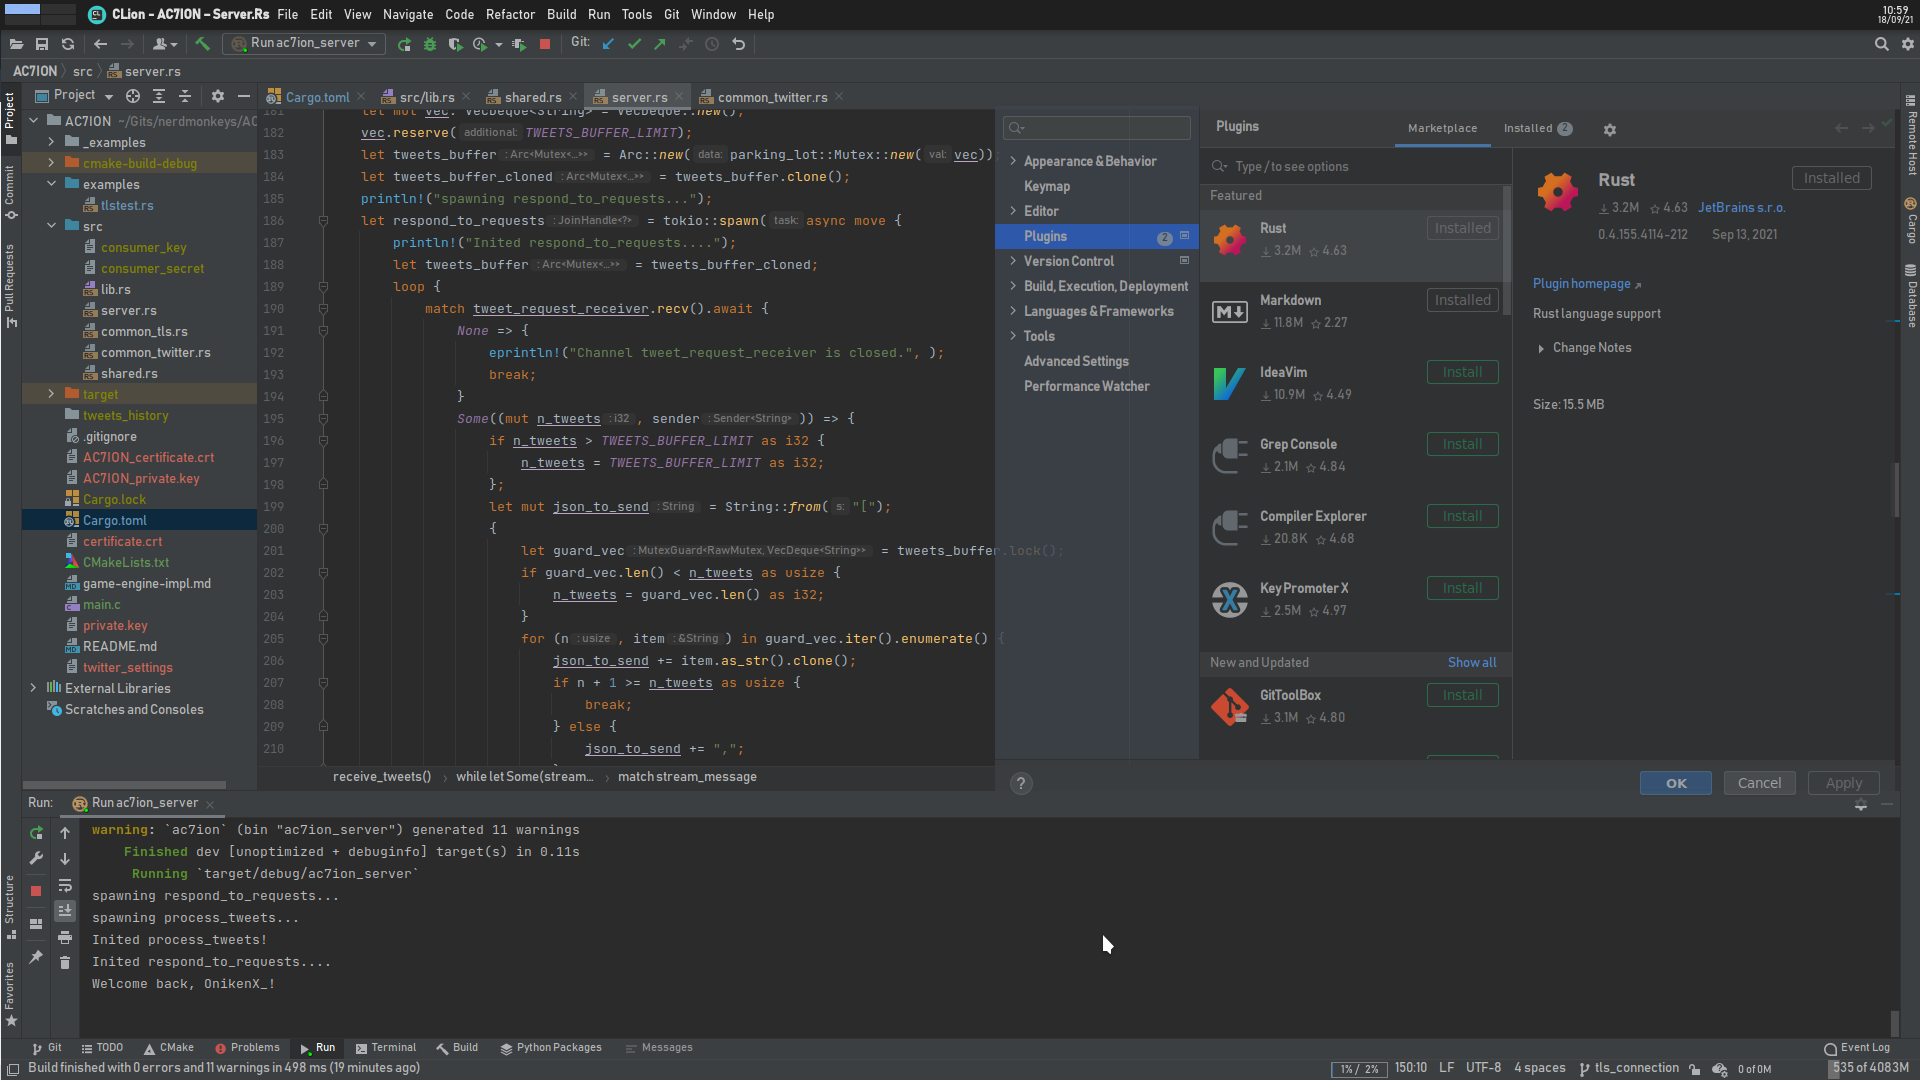
\includegraphics[width=\textwidth]{images/devenv-rust.png}
    \caption{Ambiente de desenvolvimento: \textit{Clion} com o \textit{plugin} para \textit{Rust}}
    \label{fig:devenv}
\end{figure}

\section{Arquitetura}

Usa-se um modelo servidor-cliente, em que um servidor se coneta com as \acrshortpl{api} do \gls{twitter}, recebem-se os \textit{tweets} necessários e enviam-se para os clientes que seriam bibliotecas partilhadas para os jogos usarem.

Na prática os jogos fazem o pedido de x \textit{tweets} e o cliente faz o pedido ao servidor para receber as
informações num formato de \acrshort{json}, sendo que no lado do jogo não é necessário preocupações com qualquer funcionalidade de \textit{networking}.

Na \cref{fig:twitter_arq} podemos ver de uma forma mais visual como tudo está conectado.

\begin{figure}[!ht]
  \centering
  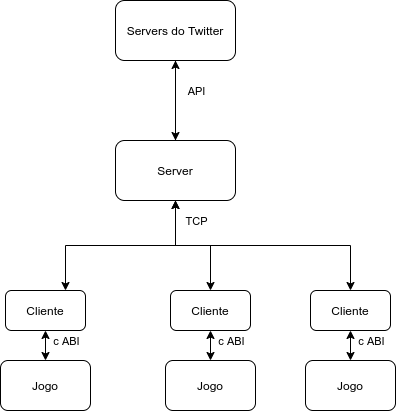
\includegraphics[width=0.9\textwidth]{twitter}
  \caption{Arquitetura do \textit{AC7ION}}
  \label{fig:twitter_arq}
\end{figure}


O server é \textit{multithreaded} e assíncrono, o que significa que ele irá usar automaticamente todos os \textit{cores} do \acrshort{cpu} do sistema em que está a ser executado. O programa também é \textit{memory safe} e não tem \glspl{data-race} já que a verificação destes problemas são verificados em tempo de compilação. \cite{rust-fearless}

\newpage
\section{Conclusão}

Com o objetivo de testar a arquitetura pretendida para o \gamechaining{}, completou-se o \textit{AC7ION} num espaço de 2 semanas. Este projeto comprovou a viabilidade desta arquitetura, proporcionando mais experiência ao estagiário em \textit{blockchain} e na criação de bibliotecas para motores de jogos de vídeo.


